\section{Mission and Objectives}
\label{sec:Introduction}
%insert image here of payload on gondola or during flight if possible.
\begin{figure}[h!]
	\begin{center}
	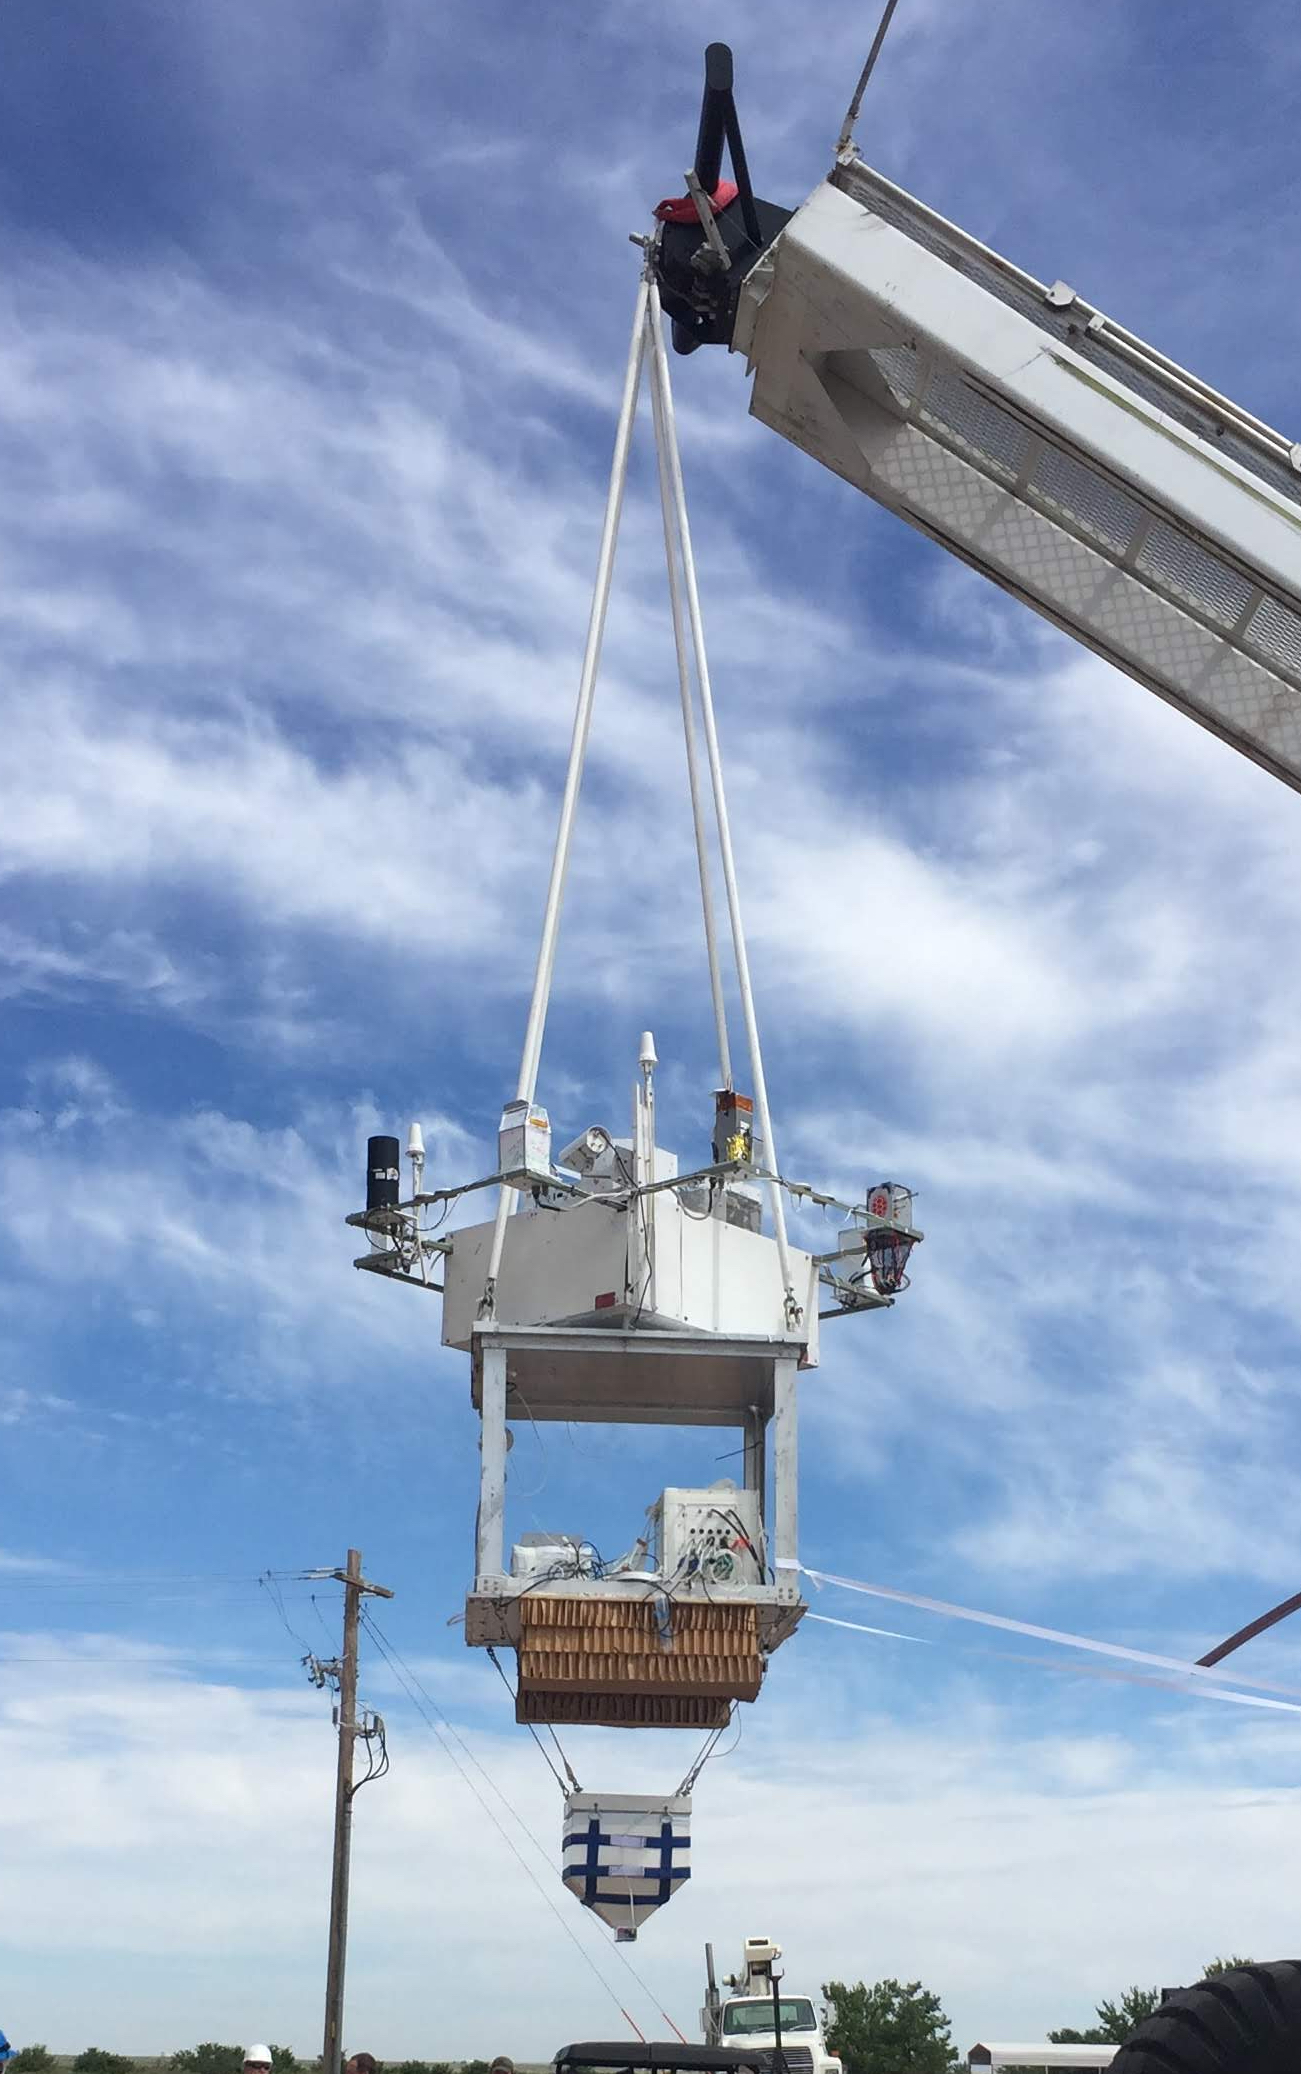
\includegraphics[width=50 mm, scale=0.5]{figures/gondola.jpg}
	\caption{Payload on the flightline}
	\label{fig:gondola}
	\end{center}
\end{figure}


%Intro (date, time, and information of general flight.  Weather conditions.  Official flight time.  Float start time and date, along with termination time and date.  Impact location.  Did it all go well?
Braving through inclement weather, SORA 2.0 took off early on September 4, 2018 at 14:03 UTC along with 12 student payloads.  From Ft. Sumner Municipal Airport, the payloads flew for approximately 9 hours.  The flight terminated at 1:31 UTC the same day and then landed shortly after at 2:11 UTC about 60 miles southwest of Mt Graham, Arizona.

%FLIGHT NUMBER: 688N
%LAUNCH TIME:09/04/2018 14:03:22 UTC
%LAUNCH LOCATION: 34.473162N 104.242232W
%FLOAT START:16:30:48 UTC
%TERMINATION:09/05/2018 01:31:23 UTC
%FLOAT TIME:09:00:35
%IMPACT:02:11 UTC
%IMPACT LOCATION:32.44816666N 109.5093472W which is 60 miles SW of Mt Graham, Arizona 

\begin{figure}[h!]
  \begin{center}
%    \begin{minipage}[c]{0.45\linewidth}
      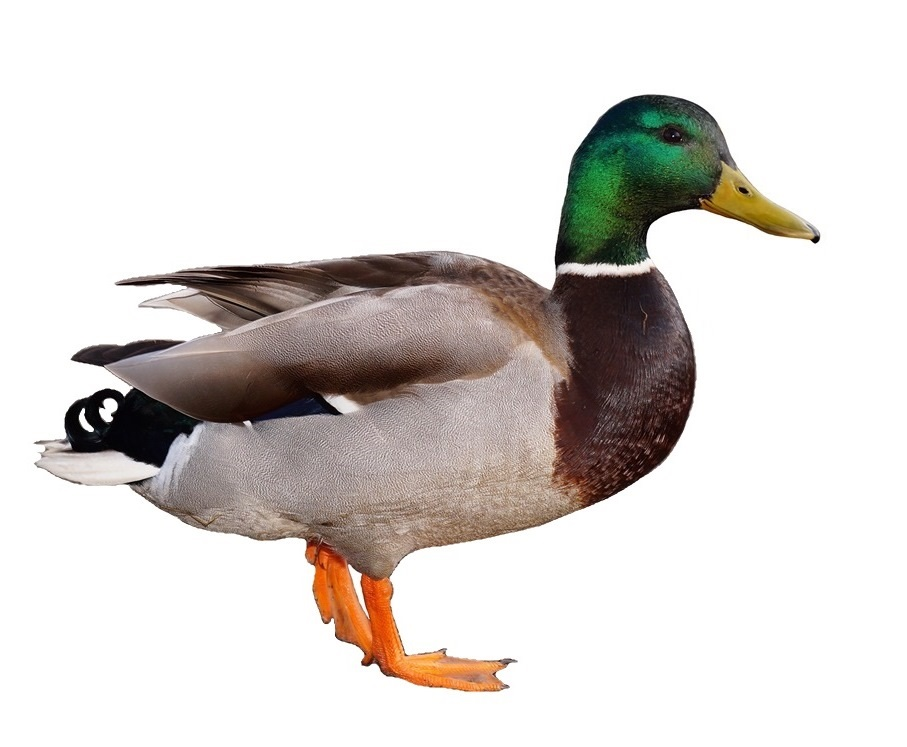
\includegraphics[width=\textwidth]{./figures/duck.jpg}
      \caption{just a duck}
      \label{fig:duck}
%    \end{minipage}
%    \hfill
%    \begin{minipage}[c]{0.49\linewidth}
%      \includegraphics[width=\textwidth]{./figures/name of figures.jpg}
%      \caption{}
%      \label{fig:}
%    \end{minipage}
  \end{center}
\end{figure}

%Mission statement and objectives:
%SORA 2.0 was a continuation of SORA~\cite{SORA} but this time seeking to . . .
SORA 2.0 was a continuation flight to further develop and build upon the first SORA flight (cite here).  To confirm and add to the findings of the first SORA flight, it was necessary to once again collect extremophile bacteria and spores that may reside 36 to 41 kilometers in the upper atmosphere.  For the radiation portion of SORA 2.0, a MiniPIX particle detector in a custom built casing was also flown to further study the surrounding radiation and the possible effects on extremophiles.  

%Did we complete our objectives?  If yes, what were they again (insert here briefly).  
%The main goals for SORA were to once again collect extremophile organisms that reside in the upper atmosphere, study the effects of surrounding radiation on these organisms in the stratosphere and gather data pertaining to the environmental conditions in which these organisms reside~\cite{SORA}.  

%From our provisional application:
%The main goals for SORA are to collect extremophile organisms that reside in the upper atmosphere, study the eects of surrounding radiation on these organisms in the stratosphere and gather data pertaining to the environmental conditions in which these organisms reside [1]. More specically, SORA has two sets of main objectives, along with four additional objectives.

SORA 2.0 Objectives here.\\
% INSERT CITATIONS HERE SINCE WE ARE TAKING FROM OUR OWN APPLICATION
{\bf Primary Objectives:}
	\begin{enumerate}
	\item Using a refined astrobiology system, attempt to capture bacteria in the upper atmosphere at approximately \SIrange{30}{41}{\kilo\meter} of altitude.
%	
%
%	Need help from Fre'Etta and Jimish here...
	\item Culture samples using (INSERT NAME OF ANALYSIS)
	\item Study the cosmic and background radiation that extromphiles may experience
	\end{enumerate}
%
%
{\bf Secondary Objectives:}
	\begin{enumerate}
	\item Develop and simplify a radiation and payload flight control system.
%	\item Determine the polar angle of hits on the detector, compare them to payload orientation information and develop simulations to verify the results.
	\item Further testing of the astrobiology hardware in flight and the methodology for collection of microbes in extreme environments at high-altitude. 
	\item Improve pre and post-flight decontamination procedures.
%Engineering Objectives
	\item Implement a variable shutter time for the MiniPIX based on the flux of particles incident on the detector.
	\item Analyze the MiniPIX data in real time and downlink relevant radiation statistics.
	\item Implement a redundant data storage mechanism.
	\item Test an improved enclosure against impacts and harsh environments.
	\item Improve astrobiology collection mechanism.
	
	\end{enumerate}

%Past scientific questions:
% Are extremophiles present in the upper atmosphere at altitudes of 36 to 41 km?  If extremophiles are captured, can the SORA payload clean box container prevent sample contamination? Finally, can we collect data accurately enough to effectively study the effects of environmental radiation on extremophile organisms and spores.
 
%New scientific questions for SORA 2.0 from provisional application:
The goals and objectives for SORA 2.0 are based on the following scientific questions: After confirming that microorganisms are present in the upper atmosphere in the first SORA mission, what extremophiles are present in the upper atmosphere at altitudes of 36 to 41 km?  If extremophiles are captured, can they be cultured and analyzed?  What methods are more effective at capturing bacteria for culturing? Finally, with a deeper understanding of the MiniPIX after the first SORA mission, can SORA 2.0 collect more data to study cosmic radiation that microoganisms and spores experience on a daily basis? Specifically, can SORA 2.0 obtain useful information about the biological effectiveness of this radiation on bacteria through parameters such as linear energy transfer and dose equivalent? 

\subsection{Hypothesis and Objectives}
\label{subsec:Hypothesis and Objectives}
\begin{enumerate}
%These are from provisional application:
%We need to review these, add more and remove some.
	\item Based on the collection results from previous HASP payloads we predict the concentration of cells at an altitude of 36 km will be less than 1000 cells per liter.
	\item Objective: Sample a minimum volumetric amount of air at target altitude for the duration of the float phase (approximately 15 to 18 hours).
	\item Based on control samples and testing before flight, we can compare our final flight results to previous applications.
	\item Objective: Quantify and characterize any contamination with our laboratory and payload disinfection procedures.
	\item Objective: Minimize the amount of external contamination before flight with thorough decontamination procedures.
	\item Based on measured results of dosage rates, the higher exposure to radiation may change the organism's cellular make-up.
	\item Objective: After capturing samples, analyze data and compare biological effects to similar genotypes found on Earth's surface.

\end{enumerate}
